%%%%%%%%%%%%%%%%%%%%%%%%%%%%%%%%%%%%%%%%%%%%%%%%%%%%%%%%%%%%%%%%%%%%%%%%%%%%%%%%%%%%
% Template for STAT 547C final project
% Author: Ben Bloem-Reddy <benbr@stat.ubc.ca>
% Date: Oct. 18, 2019
%%%%%%%%%%%%%%%%%%%%%%%%%%%%%%%%%%%%%%%%%%%%%%%%%%%%%%%%%%%%%%%%%%%%%%%%%%%%%%%%%%%%

% Note: You will get an empty bibliography warning when compiling until you include a citation.

\documentclass[10pt]{article}
% header.tex
% this is where you load pacakges, specify custom formats, etc.

\usepackage[left=1in,right=1in,top=0.75in,footskip=25pt]{geometry} 
% \usepackage{changepage}
\usepackage{amsmath,amsthm,amssymb,amsfonts}
\usepackage{mathtools}
% enumitem for custom lists
\usepackage{enumitem}
% Load dsfont this to get proper indicator function (bold 1) with \mathds{1}:
\usepackage{dsfont}
\usepackage{centernot}

\usepackage[usenames,dvipsnames]{xcolor}

% set up commenting code (I will use this during marking)
\definecolor{CommentColor}{rgb}{0,.50,.50}
\newcounter{margincounter}
\newcommand{\displaycounter}{{\arabic{margincounter}}}
\newcommand{\incdisplaycounter}{{\stepcounter{margincounter}\arabic{margincounter}}}
\newcommand{\COMMENT}[1]{\textcolor{CommentColor}{$\,^{(\incdisplaycounter)}$}\marginpar{\scriptsize\textcolor{CommentColor}{ {\tiny $(\displaycounter)$} #1}}}

\usepackage{appendix}

% set up graphics
\usepackage{graphicx}
\DeclareGraphicsExtensions{.pdf,.png,.jpg}
\graphicspath{ {fig/} }

%\usepackage[sorting=nyt,backend=biber,bibstyle=alphabetic,citestyle=alphabetic,giveninits=true]{biblatex}

\usepackage{fancyhdr}
\pagestyle{fancy}
\setlength{\headheight}{40pt}

%%%%%%%%%%%%%%%%%%%%%%%%%%%%%%%%%%%%%%%%%%%%%%%%%%%%%%%%%%%%%%%%%%%%%%%%%%%%%%%%%%%%
% most other packages you might use should be loaded before hyperref
%%%%%%%%%%%%%%%%%%%%%%%%%%%%%%%%%%%%%%%%%%%%%%%%%%%%%%%%%%%%%%%%%%%%%%%%%%%%%%%%%%%%

% Set up hyperlinks:
\definecolor{RefColor}{rgb}{0,0,.65}
\usepackage[colorlinks,linkcolor=RefColor,citecolor=RefColor,urlcolor=RefColor]{hyperref}

\usepackage[capitalize]{cleveref}
\crefname{appsec}{Appendix}{Appendices} % you can tell cleveref what to call things
% defs.tex
% this is where you define custom notation, commands, etc.


%%
% full alphabets of different styles
%%

% bf series
\def\bfA{\mathbf{A}}
\def\bfB{\mathbf{B}}
\def\bfC{\mathbf{C}}
\def\bfD{\mathbf{D}}
\def\bfE{\mathbf{E}}
\def\bfF{\mathbf{F}}
\def\bfG{\mathbf{G}}
\def\bfH{\mathbf{H}}
\def\bfI{\mathbf{I}}
\def\bfJ{\mathbf{J}}
\def\bfK{\mathbf{K}}
\def\bfL{\mathbf{L}}
\def\bfM{\mathbf{M}}
\def\bfN{\mathbf{N}}
\def\bfO{\mathbf{O}}
\def\bfP{\mathbf{P}}
\def\bfQ{\mathbf{Q}}
\def\bfR{\mathbf{R}}
\def\bfS{\mathbf{S}}
\def\bfT{\mathbf{T}}
\def\bfU{\mathbf{U}}
\def\bfV{\mathbf{V}}
\def\bfW{\mathbf{W}}
\def\bfX{\mathbf{X}}
\def\bfY{\mathbf{Y}}
\def\bfZ{\mathbf{Z}}

% bb series
\def\bbA{\mathbb{A}}
\def\bbB{\mathbb{B}}
\def\bbC{\mathbb{C}}
\def\bbD{\mathbb{D}}
\def\bbE{\mathbb{E}}
\def\bbF{\mathbb{F}}
\def\bbG{\mathbb{G}}
\def\bbH{\mathbb{H}}
\def\bbI{\mathbb{I}}
\def\bbJ{\mathbb{J}}
\def\bbK{\mathbb{K}}
\def\bbL{\mathbb{L}}
\def\bbM{\mathbb{M}}
\def\bbN{\mathbb{N}}
\def\bbO{\mathbb{O}}
\def\bbP{\mathbb{P}}
\def\bbQ{\mathbb{Q}}
\def\bbR{\mathbb{R}}
\def\bbS{\mathbb{S}}
\def\bbT{\mathbb{T}}
\def\bbU{\mathbb{U}}
\def\bbV{\mathbb{V}}
\def\bbW{\mathbb{W}}
\def\bbX{\mathbb{X}}
\def\bbY{\mathbb{Y}}
\def\bbZ{\mathbb{Z}}

% cal series
\def\calA{\mathcal{A}}
\def\calB{\mathcal{B}}
\def\calC{\mathcal{C}}
\def\calD{\mathcal{D}}
\def\calE{\mathcal{E}}
\def\calF{\mathcal{F}}
\def\calG{\mathcal{G}}
\def\calH{\mathcal{H}}
\def\calI{\mathcal{I}}
\def\calJ{\mathcal{J}}
\def\calK{\mathcal{K}}
\def\calL{\mathcal{L}}
\def\calM{\mathcal{M}}
\def\calN{\mathcal{N}}
\def\calO{\mathcal{O}}
\def\calP{\mathcal{P}}
\def\calQ{\mathcal{Q}}
\def\calR{\mathcal{R}}
\def\calS{\mathcal{S}}
\def\calT{\mathcal{T}}
\def\calU{\mathcal{U}}
\def\calV{\mathcal{V}}
\def\calW{\mathcal{W}}
\def\calX{\mathcal{X}}
\def\calY{\mathcal{Y}}
\def\calZ{\mathcal{Z}}


%%%%%%%%%%%%%%%%%%%%%%%%%%%%%%%%%%%%%%%%%%%%%%%%%%%%%%%%%%
% text short-cuts
\def\iid{i.i.d.\ } %i.i.d.
\def\ie{i.e.\ }
\def\eg{e.g.\ }
\def\Polya{P\'{o}lya\ }
%%%%%%%%%%%%%%%%%%%%%%%%%%%%%%%%%%%%%%%%%%%%%%%%%%%%%%%%%%

%%%%%%%%%%%%%%%%%%%%%%%%%%%%%%%%%%%%%%%%%%%%%%%%%%%%%%%%%%
% quasi-universal probabilistic and mathematical notation
% my preferences (modulo publication conventions, and clashes like random vectors):
%   vectors: bold, lowercase
%   matrices: bold, uppercase
%   operators: blackboard (e.g., \mathbb{E}), uppercase
%   sets, spaces: calligraphic, uppercase
%   random variables: normal font, uppercase
%   deterministic quantities: normal font, lowercase
%%%%%%%%%%%%%%%%%%%%%%%%%%%%%%%%%%%%%%%%%%%%%%%%%%%%%%%%%%

% operators
\def\P{\bbP} %fundamental probability
\def\E{\bbE} %expectation
% conditional expectation
\DeclarePairedDelimiterX\bigCond[2]{[}{]}{#1 \;\delimsize\vert\; #2}
\newcommand{\conditional}[3][]{\bbE_{#1}\bigCond*{#2}{#3}}
\def\Law{\mathcal{L}} %law; this is by convention in the literature
\def\indicator{\mathds{1}} % indicator function

% sets and groups
\def\borel{\calB} %Borel sets
\def\sigAlg{\calA} %sigma-algebra
\def\filtration{\calF} %filtration
\def\grp{\calG} %group

% binary relations
\def\condind{{\perp\!\!\!\perp}} %independence/conditional independence
\def\equdist{\stackrel{\text{\rm\tiny d}}{=}} %equal in distribution
\def\equas{\stackrel{\text{\rm\tiny a.s.}}{=}} %euqal amost surely
\def\simiid{\sim_{\mbox{\tiny iid}}} %sampled i.i.d

% common vectors and matrices
\def\onevec{\mathbf{1}}
\def\iden{\mathbf{I}} % identity matrix
\def\supp{\text{\rm supp}}

% misc
% floor and ceiling
\DeclarePairedDelimiter{\ceilpair}{\lceil}{\rceil}
\DeclarePairedDelimiter{\floor}{\lfloor}{\rfloor}
\newcommand{\argdot}{{\,\vcenter{\hbox{\tiny$\bullet$}}\,}} %generic argument dot
%%%%%%%%%%%%%%%%%%%%%%%%%%%%%%%%%%%%%%%%%%%%%%%%%%%%%%%%%%

%%%%%%%%%%%%%%%%%%%%%%%%%%%%%%%%%%%%%%%%%%%%%%%%%%%%%%%%%%
%% some distributions
% continuous
\def\UnifDist{\text{\rm Unif}}
\def\BetaDist{\text{\rm Beta}}
\def\ExpDist{\text{\rm Exp}}
\def\GammaDist{\text{\rm Gamma}}
% \def\GenGammaDist{\text{\rm GGa}} %Generalized Gamma

% discrete
\def\BernDist{\text{\rm Bernoulli}}
\def\BinomDist{\text{\rm Binomial}}
\def\PoissonPlus{\text{\rm Poisson}_{+}}
\def\PoissonDist{\text{\rm Poisson}}
\def\NBPlus{\text{\rm NB}_{+}}
\def\NBDist{\text{\rm NB}}
\def\GeomDist{\text{\rm Geom}}
% \def\CRP{\text{\rm CRP}}
% \def\EGP{\text{\rm EGP}}
% \def\MittagLeffler{\text{\rm ML}}
%%%%%%%%%%%%%%%%%%%%%%%%%%%%%%%%%%%%%%%%%%%%%%%%%%%%%%%%%%

%%%%%%%%%%%%%%%%%%%%%%%%%%%%%%%%%%%%%%%%%%%%%%%%%%%%%%%%%%
% Project-specific notation should go here
% (Because it's at the end of the file, it can overwrite anything that came before.)

%e.g.,
\def\Laplacian{\calL}
\def\P{\calP}

% combinatorial objects
\def\perm{\sigma} %fixed permutation
\def\Perm{\Sigma} %random permutation
\def\part{\pi} %fixed partition
\def\Part{\Pi} %random partition


%%%%%%%%%%%%%%%%%%%%%%%%%%%%%%%%%%%%%%%%%%%%%%%%%%%%%%%%%%
\usepackage{hyperref}
\usepackage[utf8]{inputenc}
\usepackage[english]{babel}
\usepackage{amsthm}
\theoremstyle{definition}
\newtheorem{definition}{Definition}
\newtheorem{proposition}{Proposition}
\newtheorem{theorem}{Theorem}
\newtheorem{lemma}{Lemma}
\numberwithin{equation}{section}
\usepackage{bm}
\usepackage{algorithm}
\usepackage{algpseudocode}
%\usepackage[sorting=none,backend=biber,bibstyle=alphabetic,citestyle=alphabetic,giveninits=true,natbib=true]{biblatex}
\usepackage[sorting=nyt,backend=biber,bibstyle=numeric,citestyle=numeric,giveninits=true]{biblatex}
%%%%%%%%%%%%%%%%%%%%%%%%%%%%%%%%%%%%%%%%%%%%%%%%%%%%%%%%%%%%%%%%%%%%%%%%%%%%%%%%%

% your title/author/date information go here
\title{Nonlinear state esimation method: particle filtering} % replace with your title
\author{Rachel Han} % replace with your name
\date{December 4th, 2019} % replace with your submission date
\addbibresource{../../ref/references.bib}
 % add the title of your bibliography file

% start of document
\begin{document}

\maketitle

% background section
%% !TEX root = ../main.tex

% Background section

\section{Background}



% ...


% Background section
\section{Introduction}
Nonlinear state estimation refers to estimating the true \textit{state} of a dynamic model where the underlying relationship between the \textit{observations} $(X_n)_{n \geq 1}$ (which are often corrupted versions of the \textit{state}) and the \textit{state} $(Y_n)_{n \geq 1}$ where the relationship between $X_n$ and $Y_n$ is nonlinear. There are a handful of examples listed which \cite{liu1998sequential} lists out: the states $(X_n)_{n \geq 1}$ could be unobserved signals in signal processing \cite{liu1995blind}, some characteristic of shapes observed from sequence of images \cite{blake1998statistical} and velocity of an object in a multi-target tracking problem in \cite{gordon1993novel}. These type of models where the stochastic process we are interested in is `hidden' and only inferable through some observations are called Hidden Markov Models. This term will be defined in the next section. 

We are using the notation $x_{1:n}$ for $\{ x_1, x_2, ..., x_n \}$, where $x_{1:n} \in \calX^n$.
For a filtering problem, one is interested in approximating the probability density of current state conditioned on the previous observations, $p(x_t|y_1, y_2, ..., y_t)$ at some $t$. Kalman filter is known to have a closed-form solution to this problem given that all noise is linear and Gaussian. For nonlinear state estimation problems, one can use the extended Kalman filter which linearizes about the unknown state. However, estimated the probability density function is still approximated by a Gaussian \cite{gordon1993novel}. To better approximate the underlying distribution, particle filtering (or sequential Monte Carlo) methods can be used to approximate the conditional probability density $p(x_t|y_1, y_2, ..., y_t)$. The basis of Sequential Monte Carlo (SMC) is sequential importance sampling (SIS) and resampling. SIS and resampling methods will be discussed further in later sections. First, we define Hidden Markov Models.
\subsection{Hidden Markov Model}
Let $(\Omega,\calH,\bbP)$ be a probability space. We adot the definition of Markovian process from \cite{cinlar},
\begin{definition}
	Suppose we have a stochastic process $X= (X_t)_{t \in \bbT}$  and is adapted to filtration $\calF=(\calF_t)_{t \in \bbT}$.  $X$ is \textit{Markovian with relative to} $\calF$ if for every time $t$, the past $\calF_t$ and $\calG^t_\infty = \sigma\{X_u: u \geq t, u \in \bbT \}$ are conditionally independent given the present state $X_t$.
\end{definition}
The definition says that if a process $X$ is Markovian, the future events are only determined by the present state $X_t$ and is independent of the past. We can define \textit{Hidden Markov Model (HMM)} as follows \cite{}
\begin{definition}
	Let $(X_n)_{n \geq 1}$ and $(Y_n)_{n \geq 1}$ be discrete time stochastic processes. $(X_n, Y_n)$ is a HMM if
	\begin{itemize}
		\item $X_n$ is a Markov process that is not directly observable with a initial distribution $\mu$ that describes the initial state, and the transitional kernel $K(x,B)  = \bbP(X_n \in B |  X_1 = x_1, ..., X_{n-1} = x_{n-1}) = \bbP(X_n \in B | X_{n-1}=x_{n-1})$, for $B \in \borel(\bbR^d).$ Let us call the associated density function $f(x_n|x_{n-1})$.
		\item $Y_n$ are observations whose marginal distribution is given by $\bbP(Y_n \in A| X_1 = x_1, ..., X_n = x_n) = \bbP(Y_n \in A|X_n = x_n)$, for any measurable set $A \in \borel(\bbR^d)$. Let us denote the marginal density as $g(y_n|x_n)$.
	\end{itemize}
	
	Therefore, HMM can be completely described by the initial measure $\mu$, the transition probability kernel density $f$ and the marginal density $g$.
	
\end{definition}

In the light of Baye's Theorem, according to \cite{SMCinPrac} the posterior distribution is given by
\begin{equation}
p(x_{1:n}|y_{1:n}) = \dfrac{p(y_{1:n}|x_{1:n})p(x_{1:n})}{p(y_{1:n})}.
\end{equation}
We can recursively define the evolving posterior as
\begin{equation}
p(x_{1:n+1}|y_{1:n+1}) = p(x_{1:n}|y_{1:n}) \dfrac{p(y_{n+1}|x_{n+1})p(x_{n+1}|x_{1:n})}{p(y_{n+1}|y_{1:n})}
\end{equation}
This allows us to update the posterior and predict the next state  
\begin{align}
p(x_n|y_{1:n-1}) &= \int p(x_{n}|x_{n-1})p(x_{n-1}|y_{1:n-1}) dx_{n-1} &\text{Predict}\\
p(x_n|y_{1:n}) &= \dfrac{p(y_n|x_n)p(x_n|y_{1:n-1})}{\int p(y_n|x_n)p(x_n|y_{1:n-1})} &\text{Update}
\end{align}

In general, these conditional distributions involving high dimensional integrals is hard to compute. This is why methods like Monte Carlo exist, because it allow us to approximate these quantities without having to compute the integrals, recursively. Additionally, this approximation can be done in done sequentially. This forms probabilistic dynamic system as defined in \cite{liu1998sequential}:
\begin{definition}
	A sequence of evolving probability distributions $\{\pi_n(x_{1:n})\}_{n \geq 1}$, where $n$ represents the $n$-th time step is called a probabilistic dynamic system. 
\end{definition}
Sequential Monte Carlo methods is a device to evolve the probabilistic dynamic system. For the rest of the paper, we denote the posterior $p(x_{1:n}|y_{1:n})$ as a general probability density of interest $\pi_n(x_{1:n})$, known up to a normalizing constant.
\begin{align}
\pi_n(x_{1:n}) = \dfrac{\gamma_n(x_{1:n})}{Z_n}, &{\hspace{3mm} Z_n = \int \gamma_n(x_{1:n}) d{x_{1:n}}}.
\end{align}




% add your main body sections here
\section{Perfect Sampling}

In Monte Carlo methods, we can use empirical measures to approximate the desired distribution, $\pi_n(x_{1:n})$ where $n$ represents the dimension of the probability space $\calX^n$ \cite{doucet2008}. Suppose we can sample $N$ independent and identically distributed multivariate random variables (or particles) $\{ X^{i}_{1:n}; i = 1, ..., N\}$ from the density $\pi_n(x_{1:n})$, for a fixed $n$. Given these sampled random variables, we are interested in estimating the underlying density. We can do this by using the discrete empirical measure 
\begin{equation}
	\hat{\pi}_n (x_{1:n}) = \frac{1}{N}\sum_{i=1}^{N}\delta_{X^{i}_{1:n}}(x_{1:n})
\end{equation}
Sampling directly from  $\pi_n(x_{1:n})$ is called the perfect sampling. The advantage of perfect sampling is that the variance of estimating expectation for any test function $\varphi_n$, $\var(\E[\varphi_n(x)])$, decreases as we increase the number of samples ($N$) regardless of the dimension of our probability space $\calX^n$ \cite{doucet2008}.  The variance expression is given as the following:
\begin{equation}
	\var(\E[\varphi_n(x)]) = \dfrac{1}{N} \int \varphi_n^2(x_{1:n}) \pi_n(x_{1:n})dx_{1:n} - \E[\varphi_n(x_{1:n})]^2.
\end{equation}
We can see that it decreases at a rate of $\calO(\dfrac{1}{N})$. However, sampling directly from the target distribution is not feasible since it may be complex-high dimensional. In general, generating random samples from non-standard distributions is not trivial. Additionally, our aim is to evolve the density function to accommodate the incoming data which increases the dimension of our problem each time step. Even if we were able to sample directly from the target distribution, the problem gets harder as the dimension increases \cite{doucet2008}. Therefore, we explore the following methods.

\section{Importance Sampling}

Since $\pi_n(x_{1:n})$ is difficult to sample from, one can attempt to sample from a more tractable density (easier to sample from) which is close to $\pi_n(x_{1:n})$. This is called importance sampling. We call this substitute density the importance density, denoted by $q_n(x_{1:n})$. In this paper, we outline the key ideas of important sampling explained in Doucet et al \cite{doucet2008}. We require that if $\pi_n(x_{1:n}) > 0$, then $q_n(x_{1:n}) > 0$. Importance sampling uses a simple identity. For brevity, we denote the random vector $x_{1:n}$ as $\bm{x}$. Let $\varphi(\bm{x})$ be any measurable function. Then for any test function $\varphi_n$, 
\begin{equation}
	\E_{\pi_n}[\varphi(\bm{x})]= \int_E \varphi(\bm{\bm{x}})\pi_n(\bm{\bm{x}})d\bm{x} = \left(\int_E \varphi(\bm{x}) \frac{\gamma(\bm{x})}{q_n(\bm{x})} q_n(\bm{x}) d\bm{x}\right)/Z_n = \E_{q_n}[w_n(\bm{x})\varphi(\bm{x})]/ Z_n,
\end{equation}
where $w_n$ is the unnormalised weight function and $Z_n$ is a normalising constant,
\begin{align}
	w_n(\bm{x}) &= \dfrac{\gamma_n(\bm{x})}{q_n(\bm{x})},\\
	Z_n &= \int w_n(\bm{x})q_n(\bm{x}) d\bm{x}.
\end{align}
Therefore, the target distribution is given by
\begin{equation}
	\pi_n(\bm{x}_{1:n}) = \dfrac{w_n(\bm{x})q_n(\bm{x})}{Z_n}.
\end{equation}
Assuming that $q_n(\bm{x})d\bm{x}$ dominates $\pi_n(\bm{x})d\bm{x}$ and these measures are sigma finite, we can view $w(\bm{x})$ as the Radon-Nikodym derivative. Importance sampling draws $N$ samples $X^i_{1:n} \sim q_n(x_{1:n})$. We can write down the Monte Carlo approximation of $q_n(x_{1:n})$ using the empirical measure:
\begin{equation}
	\hat{q}_n(\bm{x}) = \dfrac{1}{N}\sum_{i=1}^{N}\delta_{X^i_{1:n}}(\bm{x}).
\end{equation}
Then the approximation of the normalising constant $Z_n$ is
\begin{align}
	\hat{Z}_n = \int_E w_n(\bm{x}) q_n(\bm{x}) = \frac{1}{N}\sum_{i=1}^{N} w_n(\bm{x})
\end{align} and the target distribution $\pi_n$ is approximated by
\begin{align} \label{eq:emp_dist}
	\hat{\pi}_n(\bm{x}) = \dfrac{w(X^i_{1:n})\delta_{X^i_{1:n}}(\bm{x})}{\sum_{i=1}^{N} w_n(X^i_{1:n})}.
\end{align}
Given these approximation of distributions, we can compute approximate expectations of any test function $\varphi_n$. It is an exercise to show that estimate of the expectation of a random vector $\varphi_n(\bm{x})$ is
\begin{equation}
\E_{\hat{\pi}_n}[\varphi(\bm{x})] = \sum_{i=1}^{N} W_n^i \varphi_n(\bm{X}^i)
\end{equation}, where
\begin{equation}\label{eq:weights}
 W_n^i = \dfrac{w(X^i_{1:n})}{\sum_{i=1}^{N} w_n(X^i_{1:n})}.
\end{equation} It is important to check whether this estimate of expectation converges to the correct target $\E_{\pi_n}[\varphi_n(\bm{X}^i)]$ as $N \rightarrow \infty$. This is true indeed by law of large numbers. Furthermore, the asymptotic variance of importance sampling estimator can be given by the central limit theorem, see Theorem 1 below. A short proof of this theorem is given in \cite{geweke1989}. In this paper, with the help of \cite{impweb} we expand this proof. We state useful theorems that give the central limit theorem for importance sampling.
\begin{theorem}[Levy's Continuity Theorem] \label{levy}
	This theorem can be found in \cite{fristedt1996}. Let $\bm{X}_n = (X_{1}, X_{2}, ..., X_{k})$, and $(\bm{X})_{n \geq 1}$ be sequence of random vectors. Let $(\bm{\phi}_n(\bm{t}))_{n \geq 1}$ be the corresponding sequence of characteristic functions, where $\bm{\phi}_n(\bm{t}) = \E[e^{i\bm{t}^T\bm{X}_n}]$, for every $ \bm{t} \in \bbR^k, n \in \bbN.$ If $\phi_n(t)$ converges pointwise to its limit $\phi$: $\phi_n(t) \to \phi(t)$ then the following are equivalent:
	\begin{itemize}
		\item $\bm{X}_n$ converges in distribution to some variable $\bm{X}.$
		\item $(\bm{X}_n)_{n \geq 1}$ is tight.
		\item $\bm{\phi}(\bm{t})$ is a characteristic function of $\bm{X}$.
		\item $\bm{\phi}(\bm{t})$ is a continuous function of $\bm{t}$, and is continuous at $t=0$.
	\end{itemize}
\end{theorem} 
The proof for Levy's Continuity Theorem is omitted but can be found in \cite{fristedt1996}.

\begin{theorem}[Cramer Wold Theorem]
Let $\bm{X}_n = (X_{n1}, X_{n2}, ..., X_{nk})$ and $\bm{X} = (X_1, X_2, ..., X_k)$ be random vectors. If $\bm{t}^T \bm{X}_n \overset{D}{\to} \bm{t}^T \bar{X}$ for each $\bm{t} = (t_1, ..., t_k) \in \bbR^k$, then $\bm{X}_n \overset{D}{\to} \bm{X}$.
\end{theorem}

The proof is left as an exercise.  

\begin{theorem}[Multivariate Central Limit Theorem]
Let $\bm{X}_n = (X_{1}, X_{2}, ..., X_{k})$ be a random vector in $\bbR^k$, and each $\bm{X}_n$ be independent and identically distributed for all $n \in \{1,...,N\}$ with mean $\bm{\mu}$ and covariance $\Sigma$. Let $\bar{\bm{X}}_N = \frac{1}{N} \sum_{i=1}^{N} \bm{X}_i$. Then
\begin{equation}
	\sqrt{N}(\bar{\bm{X}}_N - \bm{\mu}) \overset{D}{\to} \calN_k(0,\Sigma), 
\end{equation}
where $\calN_k$ is the $k-$ dimensional multivariate normal distribution.
\begin{proof}
	Let $\bm{Z}_n = \bm{t}^T(\bm{X_n}-\bm{\mu})$ be a random scalar variable, and $(\bm{Z}_n)_{n \geq 1}$ be its sequence. Each $\bm{X}_n$ is independent and identically distributed with mean $\bm{\mu}$ and variance $\Sigma$. Then its affine transformation $\bm{Z}_n$ is independent and identically distributed with mean $\bm{0}$ and variance $\bm{t}^T \Sigma \bm{t}$.  The mean of $\bm{Z_n}$ is obtained by $\E[\bm{t}^T(\bm{X_n}-\bm{\mu})]= \sum_{i=1}^{N} t_i(\E[X_{ni} - \mu_i])] = 0$. The variance is $\var(\sum_{i=1}^{N} t_i(X_{ni}-\mu_i)) = \sum_{i=1}^{N} t_i^2 \var(X_{ni} - \mu_i) = \bm{t}^T \Sigma \bm{t}$. Note that the covariance terms are 0 because each $X_{n}$ is independent. Therefore, by the univariate central limit theorem $\sqrt{N}(Z_n) \overset{D}{\to} \calN(0,\bm{t}^T \Sigma \bm{t})$. Now we can apply Cramer-Wold theorem directly. Note that by the property affine transformation of multivariate normal, $ \calN(0,\bm{t}^T \Sigma \bm{t}) = \bm{t}^T \cdot \calN_k(0,\Sigma)$. Therefore, since $\bm{t}^T(\bm{X_n}-\bm{\mu}) \overset{D}{\to} \bm{t}^T \cdot \calN_k(0,\Sigma)$, $\sqrt{N}(\bar{\bm{X}}_N - \bm{\mu}) \overset{D}{\to} \calN_k(0,\Sigma)$.
\end{proof}
\end{theorem}

\begin{theorem}[Delta Method]\label{deltatheorem}
	From \cite{deltaweb}, we state the univariate delta method. Let $Y_n$ be a sequence of random variables. If for some $\theta$
	\begin{equation}
	\sqrt{n}(Y_n - \theta) \overset{D}{\to} \calN(0,\sigma^2)
	\end{equation}
	for some differentiable $g$ such that $g'(\theta) \neq 0$, then
	\begin{equation}
		\sqrt{n}(g(Y_n) - g(\theta)) \overset{D}{\to} \calN(0, \sigma^2 (g'(\theta))^2).
	\end{equation}
	\begin{proof}
		We reiterate the proof from \cite{deltaweb}. Taylor expanding $g(Y_n)$ about $\theta$, we get 
		\begin{equation}
		g(Y_n) = g(\theta) + g'(\theta)(Y_n - \theta) + \frac{g''(\theta)(Y_n - \theta)^2}{2} + \frac{g'''(\theta)(Y_n - \theta)^3}{6} + ... \nonumber
		\end{equation}
		Let $R = \frac{g''(\theta)(Y_n - \theta)^2}{2} + \frac{g'''(\theta)(Y_n - \theta)^3}{6} + ...$. Rearranging the terms and multiplying by $\sqrt{n}$,
		\begin{equation} \label{delta_eq}
		\sqrt{n}(g(Y_n) - g(\theta)) = \sqrt{n}[g'(\theta)(Y_n - \theta) + R] 
		\end{equation}
		We invoke Slutsky's theorem that we won't prove but state. The theorem states that for sequence of random variables $W_n$ and $Z_n$, if $W_n \overset{D}{\to} W$ and $Z_n \overset{prob}{\to} c$ where $c$ is a deterministic scalar, $W_n + Z_n \overset{D}{\to} W + c$ and $W_nZ_n \overset{D}{\to} cW$.
		We know by assumption, $Y_n \overset{prob}{\to} \theta $, so $\frac{g''(\theta)(Y_n - \theta)^2}{2} + \frac{g'''(\theta)(Y_n - \theta)^3}{6} + ... \overset{prob}{\to} 0$. Also $\sqrt{n}g'(\theta)(Y_n - \theta) \overset{D}{\to} \calN(0,g'(\theta)^2\sigma^2).$ This is left as an exercise to show. Then by Slutsky's theorem,
		$\sqrt{n}[g'(\theta)(Y_n - \theta) + R] \overset{D}{\to} \calN(0,g'(\theta)^2\sigma^2) + 0$, so by \eqref{delta_eq}, 
		$$ \sqrt{n}(g(Y_n) - g(\theta)) \overset{D}{\to} \calN(0,g'(\theta)^2\sigma^2). $$
	\end{proof}
	
\end{theorem}

\begin{proposition}
	\textit{Central limit theorem for importance sampling}.  Suppose $(\bm{X}_1, \bm{X}_2, ..., \bm{X}_N)$ are sequence of i.i.d random vectors. Then the following holds,
	\begin{equation}
	\sqrt{N} \left(  \sum_{i=1}^{N} W^i \varphi(\bm{X}^i) - \E_{\gamma}[\varphi(\bm{x})] \right) \overset{d}{\to} \calN(0,\sigma^2)
	\end{equation} where 
	\begin{equation}
		\sigma^2 = \int \dfrac{\gamma(\bm{x})^2}{q(\bm{x})} (\varphi(\bm{x}) - \E_{\gamma}(\varphi))^2.
	\end{equation}
	We suppress the subscript $n$ to denote the dimension, because this proposition holds for any fixed $n$. 
	
	\begin{proof}
		Let $Y_n$ be a vector \begin{equation}
		Y_N = \begin{bmatrix}
		\dfrac{1}{N}\sum_{i=1}^{N} w(\bm{X}^i)\varphi(\bm{X}^i) \\
		\dfrac{1}{N}\sum_{i=1}^{N} w(\bm{X}^i)
		\end{bmatrix}.
		\end{equation}
		Firstly, by the multidimensional Central Limit Theorem,
		\begin{equation}
			\sqrt{N}(Y_N - \E_q[Y_N]) \rightarrow \calN(0,\Sigma)
		\end{equation} as $N \rightarrow \infty$ where
		\begin{equation}
			\Sigma = \begin{bmatrix}
			\text{Var}(Y_{N,1}) & \text{Cov}(Y_{N,1}, Y_{N,2}) \\ \text{Cov}(Y_{N,2}, Y_{N,1}) & \text{Var}(Y_{N,1}).
			\end{bmatrix}.
		\end{equation} 
		The expectation of $Y_N$ can be computed as follows:
		\begin{align}
			\E_q[Y_N] &= \begin{bmatrix} \E_q[Y_{N,1}] &  \E_q[Y_{N,2}]^T \end{bmatrix}. \\
			\E_q[Y_{N,1}] &=\E_q[	\dfrac{1}{N}\sum_{i=1}^{N} w(\bm{X}^i)\varphi(\bm{X}^i)] =  \dfrac{1}{N}\E_q \left[ \sum_{i=1}^{N} \dfrac{\gamma(\bm{X}^i)}{q(\bm{X}^i)} \varphi(\bm{X}^i)\right]   \\
			&= \dfrac{1}{N}\sum_{i=1}^{N} \E_q \left[ \dfrac{\gamma(\bm{X}^i)}{q(\bm{X}^i)} \varphi(\bm{X}^i) \right] = \dfrac{1}{N} \sum_{i=1}^{N} \int \dfrac{\gamma(\bm{x}_i)}{q(\bm{x}_i)} \varphi(\bm{x}_i) q(\bm{x}_i) d\bm{x} \label{eq:finite} \\
			&= \dfrac{1}{N} \sum_{i=1}^{N} \int \gamma(\bm{x}_i) \varphi(\bm{x}^i) d\bm{x} =  \dfrac{1}{N} 
			\sum_{i=1}^{N}\E_\gamma[\varphi(\bm{\bm{X}}^i)] \overset{a.s}{\to} \E_\gamma(\varphi(\bm{x})) \label{ll_exp} 
		\end{align}
		In \eqref{eq:finite}, we care able to exchange the limit and sum because of the finiteness. \eqref{ll_exp} is by convergence of empirical distribution, $\dfrac{1}{N} 
		\sum_{i=1}^{N}\E_\gamma[\varphi(\bm{X}^i)] \overset{a.s}\to \E_\gamma(\varphi(\bm{x})) $. $\E_q[Y_{N,2}]$ can be computed similarly as
		\begin{equation}
			\E_q[Y_{N,2}] = \dfrac{1}{N}\E[\sum_{i=1}^{N} w(\bm{X}^i)] \overset{a.s}{\to} \int \gamma(\bm{x}) d\bm{x} = 1.
		\end{equation}
		Therefore, 
		\begin{equation}
			\E_q[Y_N] \overset{a.s}{\to} \left[ \E_\gamma[\varphi(x)], 1\right]
		\end{equation}
		Let $g(x,y) = \dfrac{x}{y}$ and $\mu = \E[\varphi(x)]$. Then $g(Y_N) = \sum_{i=1}^{N} W_n^i \varphi_n(X^i)$ and $g([\mu, 1]) = \mu$. The gradient $\nabla g = \left( 1/y, -x/y^2 \right).$ Therefore, by the delta method,
		\begin{equation}
			\left(  \sum_{i=1}^{N} W_n^i \varphi_n(X^i) - \mu \right) \overset{d}{\to} \calN \left( 0,\nabla g([\mu, 1])^T \cdot \Sigma \cdot \nabla g([\mu, 1]) \right).
		\end{equation}
		where $\nabla g([\mu, 1])^T \cdot \Sigma \cdot \nabla g([\mu, 1])$ can be expanded as:
		\begin{align}
		\nabla g([\mu, 1])^T \cdot \Sigma \cdot \nabla g([\mu, 1]) &= \var(Y_{N,1}) - 2\mu\covar(Y_{N,1},Y_{N,2}) + \mu^2\var(Y_{N,2})
		\end{align} By convergence of empirical distribution, as $N \to \infty$,
		\begin{align}
		\nabla g([\mu, 1])^T \cdot \Sigma \cdot \nabla g([\mu, 1]) &\overset{a.s}{\to}  \frac{1}{N}[\var(w(x)\varphi(x)) - 2\mu\covar(w(x)\varphi(x),w(x)) + \mu^2\var(w(x))] \\
		&=\frac{1}{N} \var(\mu w(x) - w(x)\varphi(x)) \hspace{1cm} \text{By property of variance of two r.v.}\\
		&= \frac{1}{N} \var((\mu - \varphi(x))w(x)) \\
		&= \frac{1}{N} [\E[w^2(x)(\mu - \varphi(x))^2] - \E[w(x)(\mu - \varphi(x))]^2] \\
		&= \frac{1}{N}(\int \dfrac{\gamma^2(x)}{q^2(x)}(\mu - \varphi(x))^2 q(x)dx - \left(\int \dfrac{\gamma(x)}{q(x)} (\mu - \varphi(x) ) q(x)dx\right)^2) \\
		&= \frac{1}{N}(\int \dfrac{\gamma^2(x)}{q(x)}(\mu - \varphi(x))^2dx - (\E_\gamma[\E_\gamma[\varphi(x)]] - \E_\gamma[\varphi(x)])^2) \\ &= \frac{1}{N} \int \dfrac{\gamma^2(x)}{q(x)}(\E_\gamma(\varphi(x)) - \varphi(x))^2dx.
		\end{align}
	
	Let $\sigma^2 = \int \dfrac{\gamma^2(x)}{q(x)}(\E_\gamma(\varphi(x)) - \varphi(x))^2dx.$. Then,
	\begin{equation}
	\left(  \sum_{i=1}^{N} W_n^i \varphi_n(X^i) - \mu \right) \overset{d}{\to} \calN \left( 0, \sigma^2 \right).
	\end{equation}
	\end{proof}

\end{proposition}

This finishes the discussion of asymptotic variance of $\E_{q_n}[\varphi_n(x)]$. Sometimes, the variance of the importance weights is of interest. The test function of interest may change every time step \cite{doucet2008}. For example, in a sequential setting, we are interested in $\varphi_{n-1}(x_{1:n-1})$ at a time step and at the next time step, $\varphi_n(x_{1:n})$. Choosing $q$ such to minimize variance of $\E_{q_n}[\varphi_{n-1}(x_{1:n-1})]$ is a bad idea. Instead, the variance of the importance weights $w_n$ independent of the test function. The expression of the variance is given below.

\begin{proposition}
	The variance of the weight function $w(\bm{x})$ is given by 
	\begin{equation} \label{eq:var_is}
	\int \dfrac{\gamma_n^2(\bm{x})}{q_n(\bm{x})} d\bm{x} - \E[\gamma_n(x)]^2
	\end{equation}
	
	\begin{proof}
		It follows from the definition of variance,
		\begin{align}
		\bbV(w(x)) &= \E_{q_n}[w^2(x)] - \E_{q_n}[w(x)]^2 \\
		&= \int \big(\dfrac{\gamma_n(\bm{x})}{q_n(\bm{x})}\big)^2 q_n(\bm{x}) dx - \left( \int \dfrac{\gamma_n(\bm{x})}{q_n(\bm{x})} q_n(\bm{x}) d\bm{x} \right)^2 \\
		&= \int \dfrac{\gamma_n^2(\bm{x})}{q_n(\bm{x})} d\bm{x} - \E[\gamma_n(x)]^2.
		\end{align}
	\end{proof}
\end{proposition} Therefore, it can be checked that the relative variance of the normalising constant is given by 
\begin{equation} \label{eq:normvar}
\dfrac{\var(\hat{Z}_n)}{Z_n^2} = \dfrac{1}{N}\left(\int \dfrac{\pi_n^2(\bm{x})}{q_n(\bm{x})} d\bm{x} - 1 \right).
\end{equation}
Observe that \eqref{eq:normvar} is minimized when $q_n = \pi_n$. Of course, making such a choice defeats the purpose of IS. Often the difficulty of this method is choosing $q_n$ such that it is close to as $\gamma_n$ as possible. 

\theoremstyle{definition}
\newtheorem{exmp}{Example}
\begin{exmp}
Here is a very simple example adapted from \cite{impint} to illustrate the idea of importance sampling. Consider the function
	\begin{equation}
		I(a) = \int_a^\infty e^{-x} dx
	\end{equation}
$f(x) = e^{-x}$ is our target density decays rapidly. We wish to compute $I(20)$. The importance sampling formulation is as follows:
\begin{equation} \label{eq:IS_example}
	\bar{I}(a) = \frac{1}{N} \sum_{i=1}^{N} \dfrac{f(X^i)}{q(X^i)}
\end{equation} for samples $X^i, i=1,...,N$ drawn from $q$. We choose a importance density $q$ such that it has a heavier tail at $x=20$ but with a similar shape. This will allow us to sample easily from the ``important" location, which is around $x=20$. Let $q$ be the pareto probability density function,
	\begin{equation}
		q(x) = \dfrac{\alpha x^\alpha_m}{x^{\alpha + 1}}.
	\end{equation}
We set the parameters to $x_m = 20$ and $\alpha = 5$. Next, we need to sample $N$ random samples from the pareto probability distribution function. We can do this by the inverse transform sampling. 
\begin{figure}[htp]
	\centering
	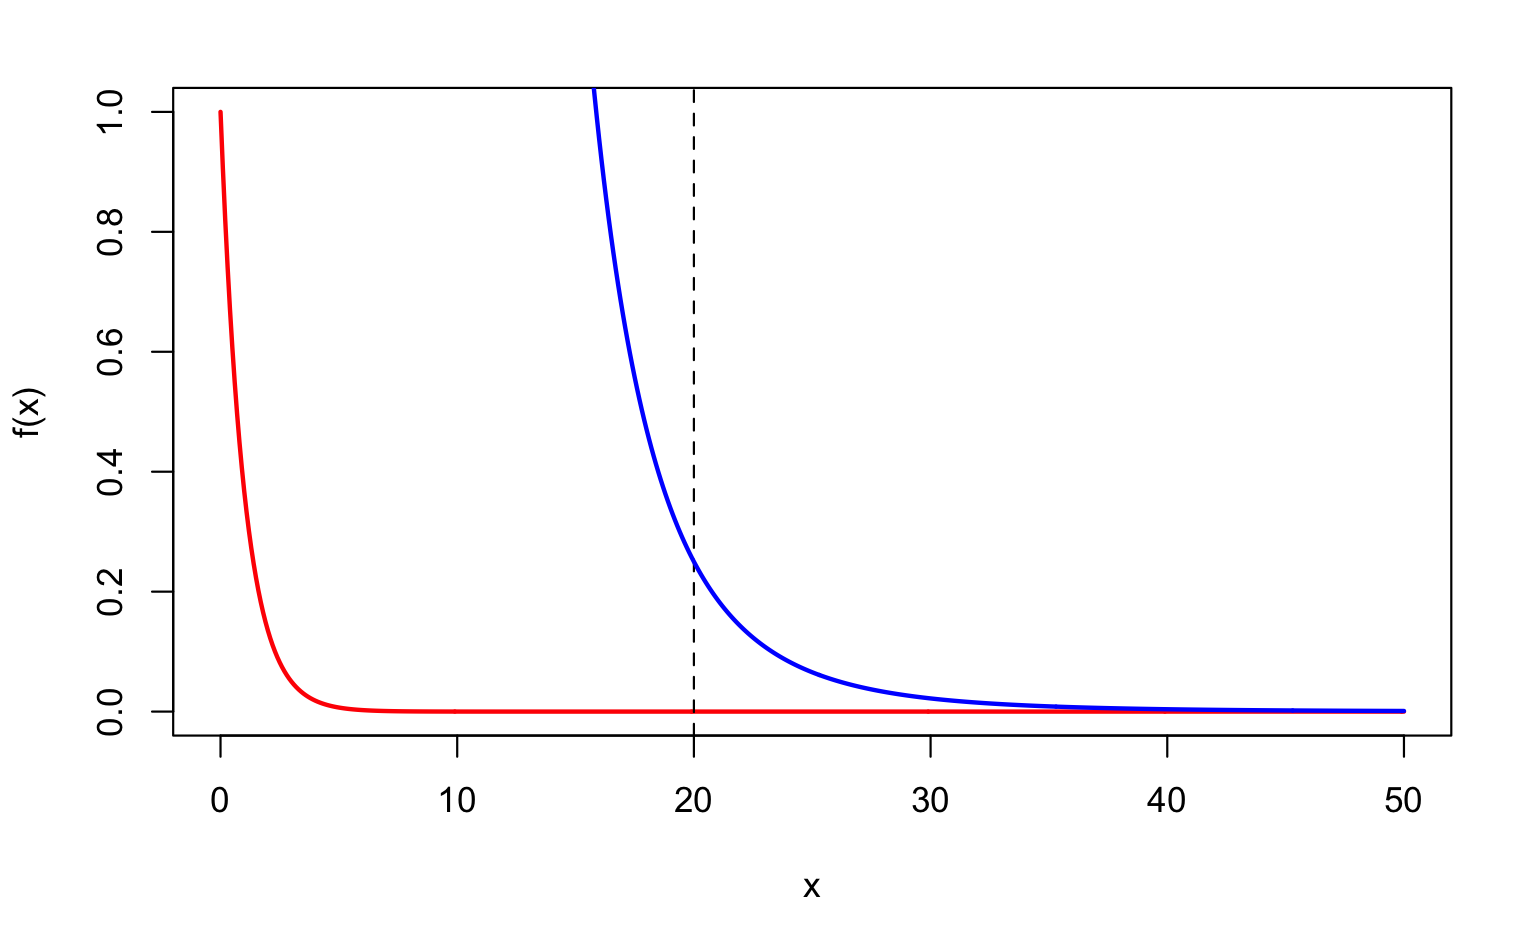
\includegraphics[scale=0.22]{target}
\end{figure}
The samples are given by 
\begin{align}
	X = \dfrac{x_m}{U^{\frac{1}{\alpha}}} &\sim \text{Pareto}(x_m,\alpha)\\	U &\sim \calU(0,1), \nonumber
\end{align} where $\calU$ is the uniform distribution.
Given $N$ samples $X^{i}$, we can compute $\bar{I(a)}$ as in Equation \eqref{eq:IS_example}. The result obtained is $\bar{I}(a) = 2.061185e-09$ and $I(a) =2.061154e-09$. We can see that $\bar{I(a)}$ approximates $I(a)$ quite well.
\end{exmp}

Importance sampling alleviates the difficulty of directly sampling from an intractable distribution $\pi_n$ by choosing a better distribution to sample from. However, note that it does not solve the problem of increasing dimensionality.
\section{Sequential Importance Sampling}

The complexity of importance sampling depends on the dimension $n$. Therefore, as the distribution evolves, the complexity of sampling from distribution will grow as a function of $n$. Sequential importance sampling (SIS) alleviates this difficulty by fixing the computational complexity at each time step. 
Many Monte Carlo problems arise where the target distribution $\pi_n$ has a decomposable structure \cite{SMCinPrac}.
\begin{align}
\pi_n(x_{1:n}) &= \pi_{n-1}(x_{1:n-1})\pi_n(x_n | x_{1:n-1}).
\end{align}
In SIS, we assume a similar structure for importance density $q_n$:
\begin{align}
	q_n(x_{1:n}) &= q_{n-1}(x_{1:n-1})q_n(x_n | x_{1:n-1}) \\
	&= q_1(x_1)\prod_{k=2}^{n}q_k(x_k|x_{1:k-1}).
\end{align} 
In SIS, we first draw a sample $X^i_1$ from $q_1(x_1)$ at time 1. Then, at time 2, we would draw the second sample $X^i_2$ from $q_2(x_2|X^i_1, X^i_2)$. At $k$-th time, one would draw $X^i_k$ from $q_k(x_k | X^i_{1:k-1})$. We would sample in this way for $i = 1, ...,N$. The unnormalised weights $w_n$ can be written recursively, 
\begin{align}
	w_n(x_{1:n}) &= \dfrac{\gamma_n(x_{1:n})}{q_n(x_{1:n})} \\
	&=\dfrac{\gamma_{n-1}(x_{1:n-1})}{q_{n-1}(x_{1:n-1})}\dfrac{\gamma_n(x_{1:n})}{\gamma_{n-1}(x_{1:n-1})q_n(x_n|x_{1:n-1})}\\
	&= w_{n-1}(x_{1:n-1})\dfrac{\gamma_n(x_{1:n})}{\gamma_{n-1}(x_{1:n-1})q_n(x_n|x_{1:n-1})}
\end{align}
Again, the variance of $w_n$ depends on the choice of $q_n(x_n|x_{1:n-1})$. From \eqref{eq:normvar}, the optimal importance density is given by $q_n^{opt}(x_n|x_{1:n-1}) = \pi_n(x_n|x_{1:n-1}) = \gamma_n(x_n | x_{1:n-1})/\int\gamma_n(x_n | x_{1:n-1})dx_n $. Then, 
\begin{equation}
	\alpha_n^{opt} = \dfrac{\gamma_n(x_{1:n-1})}{\gamma_{n-1}(x_{1:n-1})}.
\end{equation}
In most cases this optimality cannot be achieved since we do not know $\pi_n$. In the context of particle filtering, we are interested in the joint prior $p(x_{1:n}|y_{1:n})$. For simplicity, we the case consider where $\pi_n(x_{1:n}) = \gamma_n(x_{1:n}) = p(x_{1:n}|y_{1:n})$. The observations up to time $n$, $y_{1:n}$ determine the distribution at the $n$-th time. Therefore $\gamma_n(x_{1:n-1})$ correspond to $p(x_{1:n-1}|y_{1:n})$. Therefore, the optimal importance weight at time $n+1$ is given by
\begin{equation}
	w_{n+1} = w_n \dfrac{p(x_{1:n}|y_{1:n+1})}{p(x_{1:n}|y_{1:n})}.
\end{equation}
Kong et al. \cite{kong1994} showed that the sequential importance weights $w_n$ are martingales with respect to $n$ in the context of sequential imputation. Here we list out the details of this theorem in \cite{kong1994}.

\begin{theorem}[Kong-Liu-Wong Theorem \cite{kong1994}]
	The sequential importance weights $w_n$ is a martingale sequence in $n$ with random variables $x$ and $y$. This implies that the variance of the weights are increasing with respect to $n$.
	
	\begin{proof}
	Let $\calF_n$ be a filtration over the probability space $(\Omega,\calH, \bbP)$: $\calF_n = \sigma\{ x_1, x_2, ..., x_n, y_1, y_2, ..., y_n \}$. Then it is clear that for each $n\in \bbN$, $w_n \in \calF_n$, so $w)n$ is adapted to $\calF_n$. Furthermore, we assume that $\E[w_n]$ is finite. It remains to show that $\E[w_{n+1}|\calF_n] = w_n$. Since $w_n \in \calF_n$, by conditional determinism,
	\begin{equation} \label{eq:marting1}
	\E[w_{n+1}| \calF_n] = \E \left[w_n \dfrac{p(x_{1:n}|\sigma(y_{1:n}),\sigma(y_{n+1}))}{p(x_{1:n}|\sigma(y_{1:n}))} \vert \calF_n \right] = w_n\E \left[ \dfrac{p(x_{1:n}|\sigma(y_{1:n}),\sigma(y_{n+1}))}{p(x_{1:n}|\sigma(y_{1:n}))} \vert \calF_n \right].
	\end{equation} Note that the random variable of interest in \eqref{eq:marting1} is $y_{n+1}$. Let $\calG = \sigma(y_1,y_2,...,y_n), \calG_1 = \sigma(x_1,x_2,...,x_n)$ and $\calG_2 = \sigma(y_{n+1})$. Therefore, the conditional density is $p(y_{n+1}|\calG, \calG_1)$. However, $y_{n+1}$ is conditionally independent of $x_{1:n}$ given $y_{1:n}$. This is because given observations up to present time, an observation at a future time is assumed to be independent of the present states (Markov property). It is known that if for any $\sigma$-algebras $\calF, \calF_1, \calF_2$,
	\begin{equation}
	\calF_1 \condind_{\calF} \calF_2 \hspace{2mm} \text{	iff	} \hspace{2mm}  \bbP[H|\calF, \calF_1] = \bbP [H|\calF]
	\end{equation} for each $H \in \calF_2$ for the respective probability measure $\bbP$. Therefore, the conditional density is $p(y_{n+1} | \calG)$. Then, 
	\begin{align}
		\E[w_{n+1}| \calF_n] &= w_n\E \left[ \dfrac{p(x_{1:n}|\sigma(y_{1:n}),\sigma(y_{n+1}))}{p(x_{1:n}|\sigma(y_{1:n}))} \vert \calF_n \right] \\
		&= w_n \int \dfrac{p(x_{1:n}|\sigma(y_{1:n}),\sigma(y_{n+1}))}{p(x_{1:n}|\sigma(y_{1:n}))} p(y_{n+1} | \sigma(y_{1:n})) dy_{n+1} \label{eq:mart_cond}.
	\end{align}
	Again by conditional independence, $p(x_{1:n}|\sigma(y_{1:n}),\sigma(y_{n+1})) = p(x_{1:n}|\sigma(y_{1:n}))$. Therefore, since the joint distribution is the product of the marginal and conditional, $p(x_{1:n}|\sigma(y_{1:n})) p(y_{n+1}|\sigma(y_{1:n})) = p(x_{1:n},y_{n+1}|\sigma(y_{1:n})).$ Equation \eqref{eq:mart_cond} is
	\begin{align}
		\E[w_{n+1}| \calF_n] &= w_n \int \dfrac{p(x_{1:n},y_{n+1}|\sigma(y_{1:n})}{p(x_{1:n}|\sigma(y_{1:n}))} dy_{n+1} \label{eq:mart_joint} \\
		&= w_n \int p(y_{n+1}|\sigma(x_{1:n}), \sigma(y_{1:n})) dy_{n+1} &\text{Conditional is joint divided by marginal.}\\
		&= w_n \cdot 1 &\text{Integrating conditional over all $y_{n+1}$ gives 1.}
	\end{align}
	
	We have shown that $\E[w_{n+1}|\calF_n] = w_n$. It is left as an exercise to show that $\text{Var}(w_{n}) \leq \text{Var}(w_{n+1})$.
	\end{proof}
\end{theorem}

Therefore, even with $q_n^opt$, the variance of $w_n$ increases with $n$. Looking at \eqref{eq:normvar}, we see that as the importance density $q_n$ deviates from $\pi_n$, the weights $w_n$ become smaller with the growing variance. Increasing variance will drive most of the weights to zero except a few that are close to 1. The phenomenon where the weights become increasingly skewed is called the degeneracy. Although SIS can fix the dimensionality problem by restricting itself to low dimensional conditional importance densities, it cannot avoid the degeneracy when $n$ gets too large.

\section{Resampling}
The degeneracy problem can be avoided by resampling. The idea behind is that we want to make sure the particles that are likely to be sampled are kept and remove the ones with low weights. A simple resampling is called the multinomial resampling method. After sampling from the importance density $q_n$ we get the approximation of the target density \eqref{eq:emp_dist}, $$\hat{\pi}_n(x_{1:n}) = \sum_{i=1}^{N} W^i_n \delta_{X^i_{1:n}(x_{1:n})}.$$ The normalized weights $W_n^i$ from \eqref{eq:weights} are associated with each particles $X^i_{1:n}$. Multinomial resampling \cite{gordon1993novel} proceeds as follows:
\begin{enumerate}
	\item Obtain $\hat{\pi}_n$ from the samples $(X^1_{1:n}, X^2_{1:n}, ..., X^N_{1:n} )$.
	\item Sample $N$ times with replacement from $\hat{\pi}_n$ to obtain $(X^{1*}_{1:n}, X^{2*}_{1:n}, ..., X^{N*}_{1:n} ).$ According to \cite{doucet2008}, this is equal to the following:
	\begin{itemize}	
		\item Generate a random number representing the number of occurrences of each particle $N^i_n$, where it is sampled $N^i_n \sim \calM(N,w^1_{1:n},w^2_{1:n}, ..., w^N_{1:n})$. Sampling from multinomial distribution where there are $N$ possible outcomes with probability $w^i_{1:n}$ can be done in the following way. We subdivide a unit interval $[0,1]$ into $N$ pieces. Each piece is of different length proportional to some weight $w^i$ and has value $N^i$. We pick a random number from $\calU(0,1)$ which would correspond to a location on the strip. Then we return $N^i$ corresponding to the strip.
		\begin{figure}[htp]
			\centering
			
\includegraphics[scale=0.4]{tape.png}
			\caption{A visualization of multinomial sampling reduced to uniform sampling}
		\end{figure}
		
	\end{itemize}
	\item Next, we assign equal weights $1/N$ to the number of occurrences of each particle $(N^{i}_{n})_{j=1,...,N}$.
\end{enumerate}

This method works because by resampling from $\hat{\pi}_n$, we can approximate the target distribution $\pi_n$ in the limit as $N \to \infty$ as shown by Smith and Gelfand (1992). However, as shown by Chopin \cite{chopin2004central}, the local variance of estimating the expectation of a test function $\varphi_n$ is greater when we perform resampling than SIS. There are other resampling methods that attempt to reduce the variance, such as the residual resampling method by Liu and Chen \cite{liu1995blind}. In general, it is useful to resample only when there is a degeneracy because of this local variance drawback. In literature, Effective Sample Size (ESS) criterion is used to determine the degeneracy. There are many forms of ESS one can use. We present one type of ESS from \cite{liu1995blind} and \cite{kong1994}. For a fixed $n$, ESS is 
\begin{equation}
	ESS = \dfrac{N}{1+C^2(w)},
\end{equation} where $C(w)$ is the coefficient of variation
\begin{equation}
	C^2(w) = \dfrac{1}{N}\sum_{i=1}^{N} (NW^i - 1)^2.
\end{equation}
$C^2(w)$ is an approximation of the variance of importance weights when $N$ is large \cite{liu1995blind}. Large $C^2(w)$ indicates that the number of surviving samples with non-zero weights is small. Typically the threshold of ESS is set to $N/2$. 
\section{Sequential Monte Carlo}
Finally, the sequential Monte Carlo (SMC) can be articulated. A basic SMC method is Sequential Importance Resampling (SIR) which alternates between SIS and resampling. The steps of the algorithm is as follows.

\begin{algorithm}
	\caption{Sequential Monte Carlo \cite{doucet2008} }\label{SIR}
	\begin{algorithmic}[1]
		\State Sample $X^i_n$ from $q_1(x_1)$, for $i = 1, ..., N$.
		\State Compute the weights $w_1(X^i_1)$ and compute the normalized weights $W^i_1$.
		\If{ESS $< N/2$}
			\State {Resample $\{ W^i_1, X^i_1\}$  to get $\{\bar{W}^i_1, \bar{X}^i_1\} \gets \{\frac{1}{N}, X^{i*}_1\}$}
		\Else
			\State {$\{\bar{W}^i_1, \bar{X}^i_1\} \gets \{ W^i_1, X^i_1\}$.}
		\EndIf
		\For{$n=2,3,...$} 
		\State Sample $X^i_n$ from $q_n(x_n|X^{i*}_{1:n-1})$, for $i = 1, ..., N$.
		\State $X^i_{1:n} \gets \left( \bar{X}^{i}_{1:n-1}, X^i_n \right)$
		\State Compute the incremental weights $\alpha_n(X^i_{1:n})$ and the normalized weights $W^i_n \propto \bar{W}^i_n \alpha_n(X^i_{1:n})$.
		\If{ESS $< N/2$}
			\State {Resample $\{ W^i_n, X^i_{1:n}\}$  to get $\{\bar{W}^i_n, \bar{X}^i_{1:n}\} \gets \{\frac{1}{N}, X^{i*}_{1:n}\}$}
		\Else
			\State {$\{\bar{W}^i_n, \bar{X}^i_{1:n}\} \gets \{ W^i_n, X^i_{1:n}\}$.}
		\EndIf
		\EndFor
	\end{algorithmic}
\end{algorithm}
Therefore at any point in time $n$, we are able to get approximation of $\pi_n$ as $\bar{\pi}_n(x_{1:n}) = \sum_{i=1}^{N} \bar{W}_n^i \delta_{\bar{X}^{i}_{1:n}} (x_{1:n})$.


% open questions section
%% !TEX root = ../main.tex

% open questions section

\section{Open questions and research directions}
\section{Open questions and research directions}

Now that we know the theoretical justification of SMC methods, we can use it for applications of interest. A particular area I am interested in is estimating battery characteristics. For example, there is an active area of battery research devoted to create efficient estimation methods for the state of charge(SoC). The amount of charge in a battery with certain capacity is called SoC, like the battery indicator one would see on a laptop or phone (0\% to 100\% scale). One might notice that the battery indicator reflects the true SoC for a new device but as the device gets old, the estimated SoC would be less accurate. SoC cannot be measured directly but can be inferred from other measurements such as voltage and current. In fact, SoC is a function of solid lithium ion concentrations, which we denote by $c$.

Mainly, there are two battery models: equivalent circuit model and electrochemical model. The electrochemical models that describe the dynamics within the battery, which are made up of complex, deterministic partial differential algebraic equations (PDAE) to model Li-ion concentration, flux, electrolyte concentration, temperature, etc. Equivalent circuit model consists of open circuit voltage, resistor and capacitance. To formulate a particle filter problem, one would need to create a state-space model. There are different proposed state-space models from both of these models, see \cite{he2011evaluation} and \cite{tulsyan2016state}. One would need to consider the complexity of the model when selecting which dynamics to include and choosing the right parameters is not a trivial task either. 

The biggest challenge appears to be selecting the importance density. In \cite{tulsyan2016state}, the authors use Dirac distribution to satisfy the boundary conditions in their electrochemical model based particle filter approach. \cite{miao2013remaining} uses equivalent circuit model and Gaussian importance density function. However, using Gaussian may not be exploiting the full benefits particle filter that is suited for nonlinear and non-Gaussian problems. Picking a importance density that is justifiable is a crucial step in reducing the variance of the method. Then, one needs to consider the appropriate sampling technique to draw samples from the importance density. One can also experiment with various resampling methods. 

%%%% appendix
\clearpage
\appendix

% exercises and problems
% !TEX root = ../main.tex

% Exercises section

\section{Exercises}
\begin{enumerate}
	\item Show that estimate of the expectation of a random vector $\varphi_n(\bm{x})$ is
	\begin{equation}
	\E_{\hat{\pi}_n}[\varphi(\bm{x})] = \sum_{i=1}^{N} W_n^i \varphi_n(\bm{X}^i),
	\end{equation} where
	\begin{equation}\label{eq:weights}
	W_n^i = \dfrac{w(X^i_{1:n})}{\sum_{i=1}^{N} w_n(X^i_{1:n})}.
	\end{equation}
	\textit{Solution:} \\
	\begin{align}
	\E_{\hat{\pi}_n}[\varphi(\bm{x})] &= \int \varphi_n(\bm{x}) \hat{\pi}_n(\bm{x}) d\bm{x} = \int \varphi_n(\bm{x}) \hat{\pi}_n(d\bm{x}) \\
	&= \int \dfrac{w(X^i_{1:n})}{\sum_{i=1}^{N} w_n(X^i_{1:n})} \varphi_n(\bm{x}) \delta_{X^i_{1:n}}(\bm{d\bm{x}})\\
	&= \sum_{i=1}^N \dfrac{w(X^i_{1:n})}{\sum_{i=1}^{N} w_n(X^i_{1:n})} \varphi_n \circ X^i_{1:n} = \sum_{i=1}^N W^i_n \varphi_n(X^i_{1:n}).
	\end{align}
	\item Using Levy's Continuity Theorem, prove Cramer-Wold theorem:
	\begin{theorem}[Cramer Wold Theorem]
		Let $\bm{X}_n = (X_{n1}, X_{n2}, ..., X_{nk})$ and $\bm{X} = (X_1, X_2, ..., X_k)$ be random vectors. If $\bm{t}^T \bm{X}_n \overset{D}{\to} \bm{t}^T \bm{X}$ for each $\bm{t} = (t_1, ..., t_k) \in \bbR^k$, then $\bm{X}_n \overset{D}{\to} \bm{X}$.
	\end{theorem}
	\textit{Solution:} \\
	Suppose. $\bm{t}^T \bm{X}_n \overset{D}{\to} \bm{t}^T \bar{\bm{X}}$. Then, $\E[e^{i\bm{t}^T\bm{X}_n}] \overset{D}{\to} \E[e^{i\bm{t}^T\bm{X}}]$ so the characteristic functions converge. Then by Lev's continuity theorem, $\bm{X}_n \overset{D}{\to} \bm{X}$.
	\item Show that if $X_n = \sqrt{n}(Y_n - \theta)$ and $X \overset{D}{\to} \calN(0,\sigma^2)$, then  $\sqrt{n}g'(\theta)(Y_n - \theta) \overset{D}{\to} \calN(0,g'(\theta)^2\sigma^2)$, as used in the proof of multivariate central limit theorem.\\
	\textit{Solution:} \\
	Suppose $X_n \sim \calN(0,\sigma^2)$ with variance $\sigma^2$. Let $Z_n = g'(\theta)X_n$. Then $\var(Z_n) = \var(g'(\theta)X_n) = g'(\theta)^2\var(X_n) = g'(\theta)^2\sigma^2$. Since the characteristic function determines the distribution, using the fact that $\E[e^{itX_n}] = e^{\frac{1}{2}\sigma^2t^2}$, $\E[e^{itZ_n}] = \E[e^{itg'(\theta)X_n}] = \E[e^{i(tg'(\theta))X_n}] = e^{\frac{1}{2}(tg'(\theta))^2\sigma^2} $. This characteristic function of $Z_n$ is equal to that of $\calN(0,g'(\theta)^2\sigma^2)$. Therefore, $Z_n \sim \calN(0,g'(\theta)^2\sigma^2)$. So if $X_n = \sqrt{n}(Y_n -g(\theta)) \overset{D}{\to} \calN(0,\sigma^2)$ then $Z_n  =  g'(\theta)\sqrt{n}(Y_n - \theta) \overset{D}{\to} \calN(0,g'(\theta)^2\sigma^2)$. 
	\item  Show that $\text{Var}(w_{n}) \leq \text{Var}(w_{n+1})$ as a consequence of Kong-Liu-Wong Theorem.\\
	\textit{Solution:} \\
	The theorem tells us that $\var(w_n) = \var(\E[w_{n+1}|\calF_n]).$ It remains to show that $$\var(\E[w_{n+1}|\calF_n]) \leq \var(w_{n+1}).$$
	Let $(\Omega,\calH,\bbP)$ be our probability space, and let $V$ be a collection of all random variables with finite variance. $V$ is a Hilbert space with under inner product $<X,Y> = \E[XY]$, for $X, Y \in V$ \cite{zimmerman}. So $w_{n+1} \in V$. $\calF_n$ which is sigma algebra generated by a collection random variables in $V$ is a closed subspace of $V$.  $w_{n+1}$ The two variances of interest are given by:
	\begin{align}
	\var(w_{n+1}) &= \E[(w_{n+1})^2] - \E[w_{n+1}]^2, \\
	\var(\E[w_{n+1}|\calF_n]) &= \E[\E[w_{n+1}|\calF_n]^2] - \E[\E[w_{n+1}|\calF_n]]^2 = \E[\E[w_{n+1}|\calF_n]^2] - E[w_{n+1}]^2.
	\end{align}
	It remains to show that
	\begin{equation}
	\E[\E[w_{n+1}|\calF_n]^2] \leq \E[(w_{n+1})^2].
	\end{equation} 
	Writing in terms of inner product,
	\begin{equation}
	\E[\E[w_{n+1}|\calF_n]^2] = \norm{\E[w_{n+1}|\calF_n]}^2
	\end{equation}
	The conditional expectation of $w_{n+1}$ given $\calF_n$ is equivalent to the orthogonal projection of $w_{n+1}$ onto closed subspace $\calF_n$. Let $P:V \to V$ be the projection operator. Then $\E[w_{n+1}|\calF_n] = P_{\calF_n}(w_{n+1}).$ By the property of orthogonal projection,
	\begin{equation}\label{eq:proj}
		\norm{w_{n+1}}^2 = \norm{P_{\calF_n}(w_{n+1})}^2 + \norm{w_{n+1} - P_{\calF_n}(w_{n+1})}^2.
	\end{equation}
	By the projection property \eqref{eq:proj}, $\norm{w_{n+1} - P_{\calF_n}(w_{n+1})}^2 \geq 0$, $\norm{w_{n+1}}^2 = \E[(w_{n+1})^2] \geq norm{P_{\calF_n}(w_{n+1})}^2 = \E[\E[w_{n+1}|\calF_n]^2]$. 
\end{enumerate}


% any other appendix sections


% bibliography
\section{Bibliography}
\printbibliography
%\bibilographystle{plain}

\end{document}